\documentclass[12pt]{article}
\usepackage[utf8]{inputenc}
\usepackage{graphicx}
\usepackage{subcaption} %Para soportar varias figuras y leyendas dentro de un solo elemento flotante
\usepackage{tikz} %Para crear un gráfico con nodos, que incluya las imágenes y etiquetas
\title{Subfiguras con etiquetas hechas en TikZ}
\author{Curso de introducción a LaTeX}
\begin{document}
\maketitle
\begin{figure}[h]
        \centering
        \begin{subfigure}[t]{0.3\textwidth}
                \centering
                \begin{tikzpicture}
                	\node at(0,0) {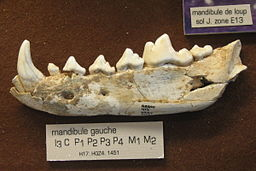
\includegraphics[width=\textwidth]{fig/mandibula}};
                	\node[white] at (-1.3,.8) {(a)};
                \end{tikzpicture}
                \phantomsubcaption\label{sf:mandibula}
        \end{subfigure}
        ~
        \begin{subfigure}[t]{0.3\textwidth}
                \centering
                \begin{tikzpicture}
                	\node at(0,0) {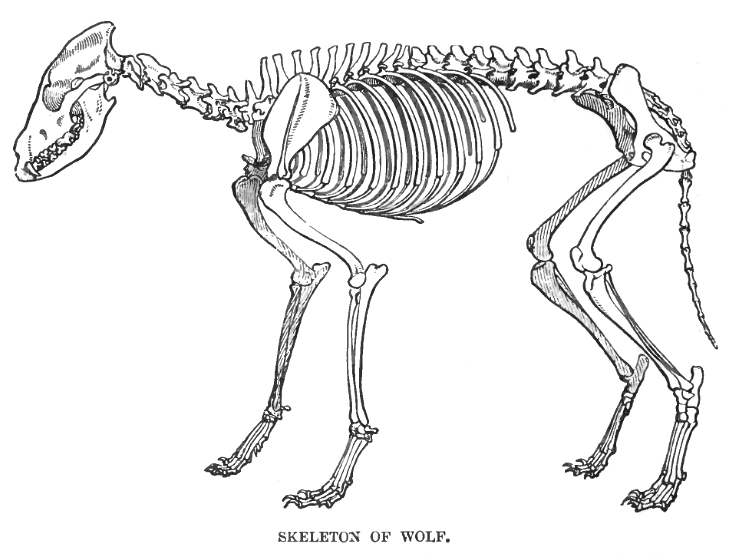
\includegraphics[width=\textwidth]{fig/esqueleto}};
					\node at (-1.2,.7) {(b)};
                \end{tikzpicture}
                 \phantomsubcaption\label{sf:esqueleto}
        \end{subfigure}
        ~
        \begin{subfigure}[t]{0.3\textwidth}
                \centering
                \begin{tikzpicture}
                	\node at(0,0) {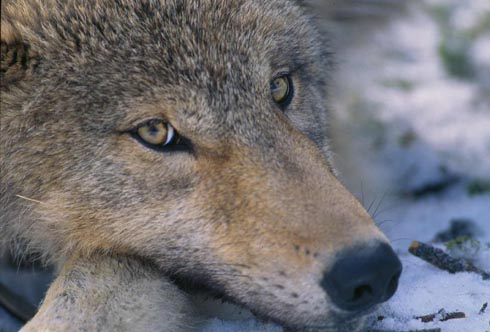
\includegraphics[width=\textwidth]{fig/closeup}};
                	\node[white] at (-1.3,.8) {(c)};
                \end{tikzpicture}
                \phantomsubcaption\label{sf:closeup}
        \end{subfigure}
        \caption{Imágenes de lobos. En \ref{sf:mandibula} vemos la mandíbula de un lobo, mientras que en \ref{sf:esqueleto} observamos la ilustración del esqueleto de un lobo. Finalmente en \ref{sf:closeup} podemos ver el acercamiento a los ojos de un lobo.}\label{fig:animals}
\end{figure}
\end{document}